\chapter{First Usability Study} \label{chapter:first-iteration}
Using the prototype described in the previous chapter a task-based usability study was performed. The goal was to evaluate whether the system could be used without prior training and how well the version control workflow could be integrated into the content authoring process.

\section{Study Design}
% general purpose of study and procedure
The purpose of this study was to evaluate whether users would be able to utilize the different version control features as part of the content authoring workflow. Additionally, the aim was to expose severe usability issues that could prevent users from getting their jobs done. Therefore, the sessions were scenario-based, which means that participants had to perform a number of tasks which reflected their everyday work. This put more emphasis on the actual behavior of users instead of opinions and attitudes and allowed the test moderator to stay in the background. This method is often referred to as \textit{assessment} or \textit{summative study} \cite{rubin_handbook_2008,goodman_observing_2012}. These kind of studies can yield more honest results because the method involves less interference than for example exploratory tests. The number of participants was kept rather small, informed by Nielsen's insight that 5 users are sufficient to find 85\% of the usability problems if the user group is more or less uniform \cite{nielsen_why_2000}.

% metrics
In addition to observing users during the scenarios, a few quantitative metrics were measured, such as task completion or error rate. Because of the small sample size, these metrics are unlikely to deliver statistically significant results, which is why they should not be relied upon alone. Nevertheless, they can serve as an indicator of potential problem areas, which could then be investigated further (e.g. in the following focus group).

% what was tested? system under test
The study was conducted using a semi-interactive prototype that was based on simple graphical layouts. The prototype was mostly black and white and only those parts that were actually needed for the user tests were interactive. It should be noted that the prototype went through several iterations before being tested. Because of its rather low fidelity, tweaking or modifying the prototype, e.g. after design feedback rounds, was relatively easy.

\subsection{Participants}
The participants were recruited randomly on a first come first serve basis. All participants were full-time employees at Babbel, but some of them had also worked as freelancers before (Table \ref{table:user-test-participants}). So, even though most of them worked as content editors at the time, they also had experience in translation, proofreading and quality assurance. This was important in order to cover all aspects of the content authoring process and test the tool regarding the different requirements of these groups.

\begin{table}[h!]
\begin{tabular}{|l|l|l|p{2cm}|p{4cm}|}
\hline
\rowcolor[HTML]{EFEFEF}
{\bf Participant} & {\bf Language Team} & {\bf Job Position} \\ \hline
1 & French & Content Editor, QA \\ \hline
2 & Portuguese & Content Editor \\ \hline
3 & Portuguese & Content Editor, Translator \\ \hline
4 & Spanish, Portuguese & Project Manager \\ \hline
5 & Turkish, German & Project Manager \\ \hline
\end{tabular}
\centering
\caption{List of Participants}
\label{table:user-test-participants}
\end{table}


% \section{Tested Feature Set}
% All features being tested were related to the version control capabilities of the new content authoring tool. It was important to test these, because they have not been part of the old CAT and furthermore they will be used very frequently. The list below shows which features have been tested exactly and how they are prioritized. All features were rated on a scale from 1-5 based on their importance and the level of doubt about the solutions. These numbers were then multiplied to get a total for each feature. One feature that was not included in the prototype is the resolution of merge conflicts. In theory this should be an edge case and therefore no resources were dedicated to it at this early stage of the interface.

% \begin{table}[h!]
% \begin{tabular}{|p{5cm}|l|l|l|}
% \hline
% \rowcolor[HTML]{EFEFEF}
% {\bf Feature Description}           & {\bf Importance} & {\bf Doubt} & {\bf Total} \\ \hline
% Editing and saving content          & 5                & 5           & 25          \\ \hline
% Creating pull requests              & 4                & 5           & 20          \\ \hline
% Creating and switching branches     & 5                & 4           & 20          \\ \hline
% Reviewing and merging pull requests & 4                & 4           & 16          \\ \hline
% View history of changes             & 3                & 4           & 12          \\ \hline
% \end{tabular}
% \centering
% \caption{Feature Prioritization}
% \label{table:feature-prio}
% \end{table}

%\section{Methodology}
%Below the methodology of the usability study is described in more detail. The tests were based on three different task scenarios. While users performed these tasks the test moderator as well as two observers took notes. Furthermore the sessions were recorded so that time for task completion could be measured as well as the error rate.

% here should be more about tasked-based user studies and why it was decided to do this

% \section{Test Objectives}
% There were several questions that should be answered with the user test:

% \begin{itemize}
%   \item Evaluate whether users appreciate the separation of editing and saving or if they experience it as a burden.
%   \item To observe how users react to the fact that they have to describe their changes when saving.
%   \item Evaluate whether the concept of a branch is understood and can be used in a meaningful way by users.
%   \item Evaluate whether users are able to use pull requests in a meaningful way.
%   \item Evaluate whether the history of changes gives users a good idea about what kind of changes happened recently.
%   \item Observe which concepts and terms confuse users the most.
% \end{itemize}

\subsection{Metrics}
Even though these quantitative measures are not statistically significant with a group of just 5 participants, they can still hint at potential problems, which should be investigated further.

% phrase it nicer, statistically significant

\begin{itemize}
  \item \emph{Successful Task Completion}: percentage of tasks that were completed successfully
  \item \emph{Time On Task}: time that was needed to perform a task
  \item \emph{Error Rate}: participant deviated from “ideal” path of navigation, such as opening the wrong menu.
\end{itemize}

%What counts as an error??

\subsection{Scenarios} \label{sec:scenario-descriptions}
As suggested by Nielsen Norman Group the tasks given to the participants were situated within real-world scenarios \cite{_task_2014}. This usually makes it easier for participants to engage with the interface in a realistic way. Furthermore, when some context is provided, the task itself does not need to be described as detailed, but rather the end-goal can be defined and the means of achieving this end-goal can be left open for the user. Three different task scenarios with an estimated duration of 4-8 minutes were created. The following task scenarios were given to the participants.

\subsubsection{Scenario 1: Fix Error and Allow Review}
A colleague (Firstname Lastname) has sent you a link to a lesson. She informed you that the second item in the vocabulary (write) exercise has the wrong speaker role (should be F1) and also should be added to the review manager. She asked you to correct the error and afterwards allow her to review your changes. Make sure you are not editing the live content.

% \begin{itemize}
%   \item End goal: Let colleague review changes
%   \item Link: https://marvelapp.com/c89590
% \end{itemize}

\subsubsection{Scenario 2: Publish Changed Content}
A colleague (Firstname Lastname) has changed a lesson within the German language package. She asked you to review the changes. Look at the changes she made and if you do not find any errors make them available to the Babbel end-user.

% \begin{itemize}
%   \item End goal: Publishing changed content
%   \item Link: https://marvelapp.com/1011fjj
% \end{itemize}

\subsubsection{Scenario 3: Eliminate Error and Save}
A translator (user name) is currently working on a localization of German lessons (to Portuguese). Recently a translated exercise was published, but according to customer service users have complained that there is a translation missing within this exercise. Find the exercise which has been translated and locate the item with the missing translation. Add the translation and save your changes.

\subsection{Sessions}
In the beginning of each session the participant received a short introduction to the reasons behind the study and the procedure of the session. In order to make him or her feel more comfortable, it was highlighted that the interface was being tested and not the participant. Each session was structured into three different parts: First, a short questionnaire had to be answered, then the participant had to go through the three different scenarios (as described above) and lastly, he or she was asked some follow-up questions and encouraged to provide feedback on the interface. While performing these tasks, participants were asked to think aloud, especially when running into problems. During each session the author was present as test moderator as well as one or two observers who took notes. The sessions usually took no longer than 30 to 45 minutes.

\section{Findings}
The results below are structured in the same way the testing sessions were. First, the results of the questionnaire are presented. Then, the quantitative metrics, recorded during the sessions, are shown in four different tables. In the end, problems that became apparent when observing the participants, are listed and described in detail.

% \subsection{Pre-session Questionnaire}
% The pre-session questionnaire consisted of four different questions, that were intended to evaluate the user’s experience with version control, the current CAT and other content management or authoring systems. The table shows that no participant had prior knowledge of version control and only one had used another content management system besides the content authoring tool of Babbel. Furthermore, three out of five participants had one to three years experience with the CAT. One had less than a year of experience and one had more than three years experience. A summary of this data can be found in the appendix (Table \ref{table:pre-sess-quest}).

\subsection{Metrics}
Several quantitative metrics were gathered during the user sessions. These include completion rates, error rates and time needed for the scenarios. The metrics serve as an add-on for the mostly qualitative user studies and help to interpret the observations and findings of the test sessions.

\subsubsection{Task Completion Rate}
The table below shows a summary of how many scenarios have been successfully completed. The completion rates for Scenario 1 and Scenario 3 could hint at potential problems, which are further discussed below.

\begin{table}[h!]
\begin{tabular}{|l|l|l|l|}
\hline
\rowcolor[HTML]{EFEFEF}
{\bf User}                     & {\bf Scenario 1} & {\bf Scenario 2} & {\bf Scenario 3} \\ \hline
1                              & no           & yes          & yes          \\ \hline
2                              & yes          & yes          & yes          \\ \hline
3                              & yes          & yes          & no           \\ \hline
4                              & no           & yes          & no      \\ \hline
5                              & no      & yes          & yes          \\ \hline
\rowcolor[HTML]{EFEFEF}
Success & 2 & 5 & 3 \\ \hline
\rowcolor[HTML]{EFEFEF}
{\bf Completion Rate} & {\bf 40\%}   & {\bf 100\%}  & {\bf 60\%}   \\ \hline
\end{tabular}
\centering
\caption{Task completion rate}
\label{table:task-completion-rate}
\end{table}

\subsubsection{Time on Task}
The time on task was measured based on the video recordings of the sessions. The large differences between Scenario 2 and the other scenarios might be due to the different levels of difficulties inherent to the tasks presented in the scenarios. The table below highlights the different durations (in seconds) that were needed to finish a certain scenario. The mean for Scenario 1 has the highest \ac{SD}, which could point towards potential usability problems which were not encountered by all users. Scenario 1 asked users to “not edit the live data”, which meant that they had to create a new branch. Since none of the participants had prior experience with version control, this was a particularly difficult scenario for some of them.

\begin{table}[h!]
\begin{tabular}{|r|r|r|r|r|r|r|r|}
\hline
\rowcolor[HTML]{EFEFEF}
{\bf Scenario} & \multicolumn{1}{c|}{\cellcolor[HTML]{EFEFEF}{\bf User 1}} & {\bf User 2} & {\bf User 3} & {\bf User 4} & {\bf User 5} & {\bf Mean} & {\bf SD} \\ \hline
\cellcolor[HTML]{EFEFEF} 1 & 505 & 270 & 313 & 275 & 519 & 376 & 133.1 \\ \hline
\cellcolor[HTML]{EFEFEF} 2 & 81 & 226 & 73 & 170 & 90 & 128 & 67.2 \\ \hline
\cellcolor[HTML]{EFEFEF} 3 & 301 & 375 & 418 & 507 & 399 & 400 & 85.2      \\ \hline
\end{tabular}
\centering
\caption{Time needed to perform scenarios (in seconds)}
\label{table:time-on-tasks}
\end{table}

\subsubsection{Error Rates}
An interaction was counted as an error if the user departed from the ideal path and thus the interaction did not contribute to solving the overall goal of the scenario. The table below helps to paint a picture of how much trial and error was necessary. The error rate is not necessarily a sign for bad usability, it can also reflect the difficulty of a scenario. For example, Scenario 1 and 3 involved using similar parts of the interface, but Scenario 3 challenged a participant's mental model of the system whereas Scenario 1 was a little more straightforward.

% explain how mental model was challenged

\begin{table}[h!]
\begin{tabular}{|r|r|r|r|r|r|r|r|}
\hline
\rowcolor[HTML]{EFEFEF}
\multicolumn{1}{|l|}{\cellcolor[HTML]{EFEFEF}\textbf{Scenario}} & \multicolumn{1}{l|}{\cellcolor[HTML]{EFEFEF}\textbf{User 1}} & \multicolumn{1}{l|}{\cellcolor[HTML]{EFEFEF}\textbf{User 2}} & \multicolumn{1}{l|}{\cellcolor[HTML]{EFEFEF}\textbf{User 3}} & \multicolumn{1}{l|}{\cellcolor[HTML]{EFEFEF}\textbf{User 4}} & \multicolumn{1}{l|}{\cellcolor[HTML]{EFEFEF}\textbf{User 5}} & \multicolumn{1}{l|}{\cellcolor[HTML]{EFEFEF}\textbf{Mean}} & \multicolumn{1}{l|}{\cellcolor[HTML]{EFEFEF}\textbf{SD}} \\ \hline
\cellcolor[HTML]{EFEFEF}1 & 3 & 1 & 3 & 3 & 1 & 2.2 & 1.1 \\ \hline
\cellcolor[HTML]{EFEFEF}2 & 0 & 5 & 0 & 3 & 0 & 1.6 & 2.3 \\ \hline
\cellcolor[HTML]{EFEFEF}3 & 3 & 6 & 7 & 3 & 2 & 4.2 & 2.2 \\ \hline
\end{tabular}
\centering
\caption{Number of errors by each participant}
\label{table:error-rate}
\end{table}

\subsection{Discovered Usability Issues} \label{sec:usability-issues-1st-study}
The following section describes the usability issues that were discovered by observing participants during the sessions. In total, 26 different problems were identified. 7 of them were of the highest severity, preventing participants from finishing their tasks. 8 issues caused a significant delay or frustration for users. The remaining issues only caused minor problems or were suggestions for improvement.

In order to rank the issues by their impact on the user experience, a combination of severity and frequency was used to derive an impact score. The severity of each problem was determined based on four different definitions \cite{sauro_quantifying_2012}:

\begin{itemize}
\item 10 points: Severe usability issues preventing users from completing the task scenarios
\item 5 points: Usability issues causing a significant delay or frustration
\item 3 points: Minor usability issues which are merely a nuisance
\item 1 point: Improvements suggested by participants
\end{itemize}

To calculate the impact score the severity was multiplied by the frequency of users who experienced the problem (severity * frequency / 10). A frequency of 40\% means that 4 of 10 users encountered the problem, independent of whether they ran into the issue more than once. The scale ranges from 100 (most severe problem, experienced by all users) to 1 (suggestion by a single user).

The issues below are grouped by feature areas and ranked by their impact on the user experience. Issues with a high impact are shortly explained.

\subsubsection{Branches}
As can be seen in Table \ref{table:issues-branches} one of the most impactful usability issues was the difficult discovery of the branch creation functionality (Issue \#1). During Scenario 1, 3 out of 5 participants spent more than half of the time by searching for this feature. Figure \ref{fig:branch-creation-time} visualizes this fact. The dark bars mark the point in time when users discovered the branch creation feature. The problem might have been a missing label for the button, which only consisted of a plus sign. Apparently, the proximity to the branch dropdown as well as the tooltip appearing upon hovering the button, did not suffice to make this feature discoverable.

There were two more issues with a severity score of 10. Issue \#2: Some users dismissed the master branch warning (without reading it), which lead to even more confusion and prevented some of them from finishing the task.

The remaining issues highlight that the concept of a branch was only poorly understood (Issue \#3) and that the naming of the default branch (master) is rather unfortunate (Issue \#4), because it interferes with a different concept (master language) that describes the main translation language.

\begin{table}[h!]
\centering
\begin{tabular}{|l|p{7cm}|l|l|l|}
\hline
\rowcolor[HTML]{EFEFEF}
\textbf{\#} & \textbf{Usability issue} & \textbf{Severity} & \textbf{Frequency} & \textbf{Impact} \\ \hline
1 & Create new branch button was not found & 10 & 40\% & 40 \\ \hline
2 & Warning about editing content inside the master branch was ignored & 10 & 40\% & 40 \\ \hline
3 & It is not clear that the master branch represents the public content and the content in all other branches is not visible to the end-user. & 5 & 60\% & 30 \\ \hline
4 & The naming for the master branch was confused with the concept of a master language. & 5 & 40\% & 20 \\ \hline
5 & After creating branch it is not clear that system switched to new branch already & 5 & 20\% & 10 \\ \hline
\end{tabular}
\caption{Usability problems related to branches}
\label{table:issues-branches}
\end{table}

\begin{figure}[h!]
 \centering
 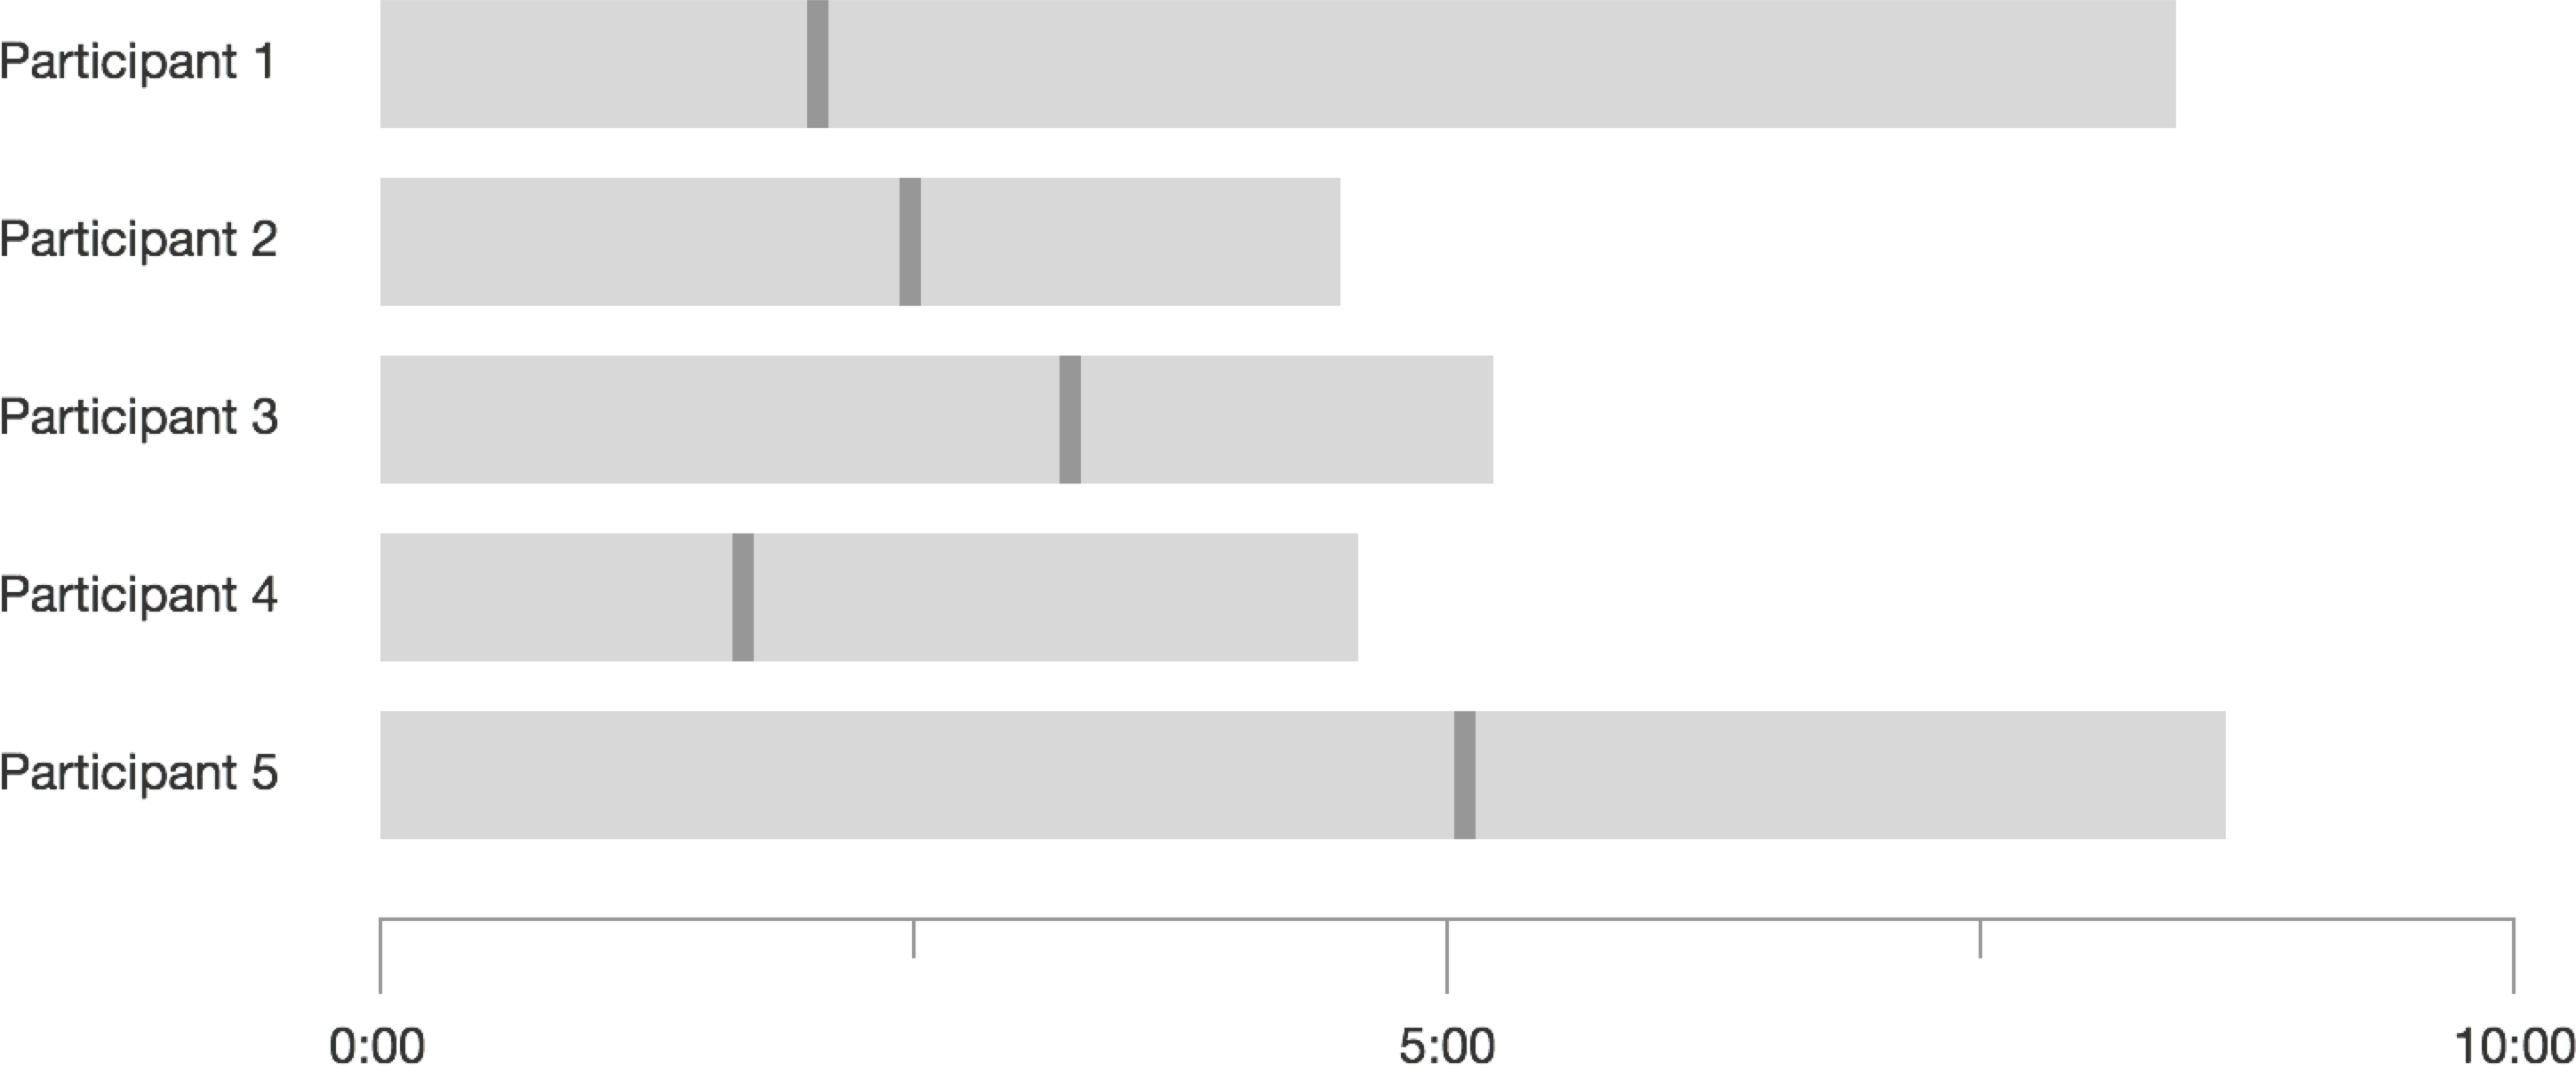
\includegraphics[width=12cm]{plot-time-till-branch-creation}
 \caption{Total task completion time compared to discovery of branch creation button}
 \label{fig:branch-creation-time}
\end{figure}

\subsubsection{Pull Requests}
Pull requests are similar to branches in that they are one of the most complex concepts in version control. As suspected, they caused a couple of usability problems. The most important issue was related to the naming: deriving the functionality of a pull request just from its name is almost impossible (Table \ref{table:issues-pull-requests}, Issue \#6). When using a Git CLI the \emph{pull} command fetches changes from the remote repository and merges them into the local repository. Therefore, a pull request describes a request to "pull a new set of changes". But since this command is not exposed to users inside the GUI of the content authoring tool, it is fairly difficult for them to guess what kind of functionality is concealed behind this name.

\begin{table}[h!]
\centering
\begin{tabular}{|l|p{7cm}|l|l|l|}
\hline
\rowcolor[HTML]{EFEFEF}
\textbf{\#} & \textbf{Usability issue} & \textbf{Severity} & \textbf{Frequency} & \textbf{Impact} \\ \hline
6 & Concept of a pull request is not clear (term might be confusing) & 5 & 80\% & 40 \\ \hline
7 & Some users missed the reviewer field & 10 & 20\% & 20 \\ \hline
8 & Confused pull request title with lesson title & 5 & 20\% & 10 \\ \hline
9 & Branch visualization is unclear (release branch) & 3 & 20\% & 6 \\ \hline
10 & Changes vs. Overview unclear (pull request detail view) & 3 & 20\% & 6 \\ \hline
\end{tabular}
\caption{Usability issues related to Pull Requests}
\label{table:issues-pull-requests}
\end{table}

\subsubsection{Diff}
During Scenario 3, a high proportion of users had problems comprehending the list of changes presented to them (Table \ref{table:issues-diff}, Issue \#11). In general, the diff view worked well, but when asked to find a missing translation, most users had a hard time understanding that something that had not been changed, would not appear in the diff view. Furthermore, the list of changes they did see, was confusing, because it showed empty fields, which some users mistook as the missing translation they were supposed to find (Figure \ref{fig:add-translation-diff}).

\begin{figure}[h!]
 \centering
 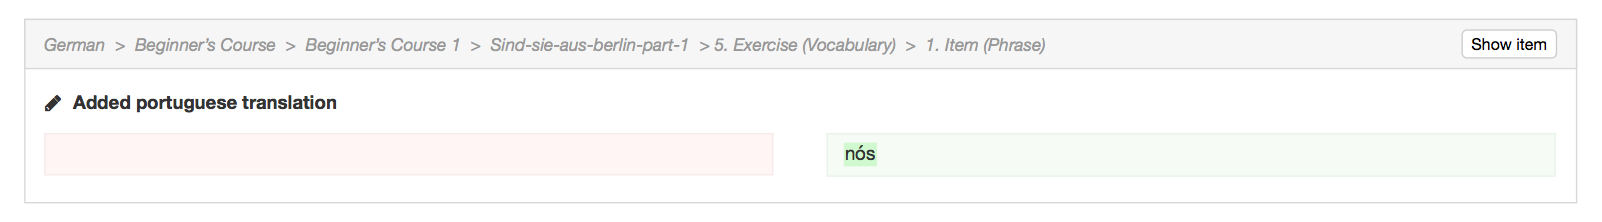
\includegraphics[width=\textwidth]{first-prototype/add-translation-diff}
 \caption{Part of diff view that displays an added translation}
 \label{fig:add-translation-diff}
\end{figure}

\begin{table}[h!]
\centering
\begin{tabular}{|l|p{7cm}|l|l|l|}
\hline
\rowcolor[HTML]{EFEFEF}
\textbf{\#} & \textbf{Usability issue} & \textbf{Severity} & \textbf{Frequency} & \textbf{Impact} \\ \hline
11 & New translations listed in the diff view are confusing, because the left column is empty (some users expected to see the learning language text) & 10 & 80\% & 80 \\ \hline
12 & Not clear how to get from the diff view to the editing view & 10 & 40\% & 40 \\ \hline
13 & red and green are confusing as colors (red is associated with a mistake) & 3 & 20\% & 6 \\ \hline
\end{tabular}
\caption{Usability issues related to the diff view}
\label{table:issues-diff}
\end{table}


\subsubsection{Saving Process}
The most problematic issue related to saving was the non-existing save button at the bottom of the view (Table \ref{table:issues-saving-process}, Issue \#14). Most users overlooked the saving feature in the navigation bar. It seems like most users would rather expect it to be attached to the lesson editor itself. The reason it is at the top is that saving is independent of content itself. In theory, several lessons could be edited and then only saved in the end altogether. This approach is very similar to how version control usually works, but it did not seem to resonate with most users. Many were anxious to navigate away from the current view after doing changes, because they feared losing the changes. In most interfaces, saving is directly associated with a change that was done before. A solution needs to be found that is less counter-intuitive, but which still offers users a way of reviewing what was changed.

\begin{table}[h!]
\centering
\begin{tabular}{|l|p{7cm}|l|l|l|}
\hline
\rowcolor[HTML]{EFEFEF}
\textbf{\#} & \textbf{Usability issue} & \textbf{Severity} & \textbf{Frequency} & \textbf{Impact} \\ \hline
14 & Save button was not found (expected at bottom of screen) & 10 & 80\% & 80 \\ \hline
15 & Expects saved changes to be public right away & 10 & 20\% & 20 \\ \hline
16 & Confused back-to-editor-button with review functionality & 5 & 40\% & 20 \\ \hline
17 & Wording on saved changes confirmation page is somewhat confusing & 3 & 20\% & 6 \\ \hline
18 & Concept of separated saving not entirely clear (across lessons) & 3 & 20\% & 6 \\ \hline
\end{tabular}
\caption{Usability issues related to the saving process}
\label{table:issues-saving-process}
\end{table}

% \subsubsection{History}
% \begin{table}[h!]
% \centering
% \begin{tabular}{|p{7cm}|l|l|l|}
% \hline
% \rowcolor[HTML]{EFEFEF}
% \textbf{Usability Issue} & \textbf{Severity} & \textbf{Frequency} & \textbf{Impact} \\ \hline
% History is not recognized for what it is. Most users take long to find it. (naming might not be obvious) & 5 & 40\% & 20 \\ \hline
% Difference between pull request and history not entirely clear & 3 & 20\% & 6 \\ \hline
% Change of a specific user is not found – search functionality suggested & 3 & 20\% & 6 \\ \hline
% \end{tabular}
% \caption{Usability issues related to the saving process}
% \label{table:issues-saving}
% \end{table}

\subsubsection{Main Editing View}
The main editing view only caused a couple of minor problems. First and foremost, the way the content was structured and presented to the user was not the most intuitive (Table \ref{table:issues-editing-view}, Issue \#19). Most users struggled with envisioning how the representation would translate into the actual exercises provided to the Babbel end-user. Additionally, the design did not provide a very good overview, because every exercise or item had to be expanded and at any given moment one could only see one at most.

The remaining issues were suggestions (Issue \#21 \& Issue \#22) or related to the visual design of the interface (Issue \#20).

\begin{table}[h!]
\centering
\begin{tabular}{|l|p{7cm}|l|l|l|}
\hline
\rowcolor[HTML]{EFEFEF}
\textbf{\#} & \textbf{Usability issue} & \textbf{Severity} & \textbf{Frequency} & \textbf{Impact} \\ \hline
19 & Visual representation/hierarchy of items/exercises not entirely clear & 3 & 60\% & 18 \\ \hline
20 & Learning language text is overlooked (looks different than translations) & 3 & 20\% & 6 \\ \hline
21 & Suggested a search functionality to find content faster & 1 & 40\% & 4 \\ \hline
22 & Suggested pro-active system for translations & 1 & 20\% & 2 \\ \hline
\end{tabular}
\caption{Usability issues related to the main editing view}
\label{table:issues-editing-view}
\end{table}


\subsubsection{Miscellaneous}
In addition to the issues related to the major feature areas a couple of miscellaneous problems appeared throughout the system. None of the issues was of the highest severity, but they still caused some frustration. Especially Issues \#23 and \#25 reduced the smoothness with which users could move through the system. It seems that the naming for some of the navigation items was not descriptive enough and that icons without a label were more or less ignored. Some users proceeded by trial and error, which does not speak for the clarity of the information architecture.

\begin{table}[h!]
\centering
\begin{tabular}{|l|p{7cm}|l|l|l|}
\hline
\rowcolor[HTML]{EFEFEF}
\textbf{\#} & \textbf{Usability Issue} & \textbf{Severity} & \textbf{Frequency} & \textbf{Impact} \\ \hline
23 & Main navigation not completely obvious, clicking through (trial \& error) & 5 & 40\% & 20 \\ \hline
24 & History is not recognized for what it is. Most users take long to find it. (naming might not be obvious) & 5 & 40\% & 20 \\ \hline
25 & Navigation: Icons without text are not understood "What is this?" (pull request icon) & 3 & 20\% & 6 \\ \hline
26 & No help offered when needed & 1 & 20\% & 2 \\ \hline
\end{tabular}
\caption{Miscellaneous usability issues}
\label{table:issues-misc}
\end{table}


% \subsubsection{Scenario 1}
% Scenario 1 asked participants to fix two errors in a lesson, save the changes and enable a colleague to review the changes before making them public. Translated into the version control world this corresponds to creating a branch, editing, staging and committing the changes and finally creating a pull request.

%The first step, creating a new branch, seemed to be the major hurdle for most participants. Even though it was basically the first thing that users had to do, 3 out of 5 participants needed more than half of the total task completion time for discovering this feature. Figure \ref{fig:branch-creation-time} visualizes this fact. The dark bars mark the point in time when users discovered the branch creation feature.

% \begin{figure}[h!]
%  \centering
%  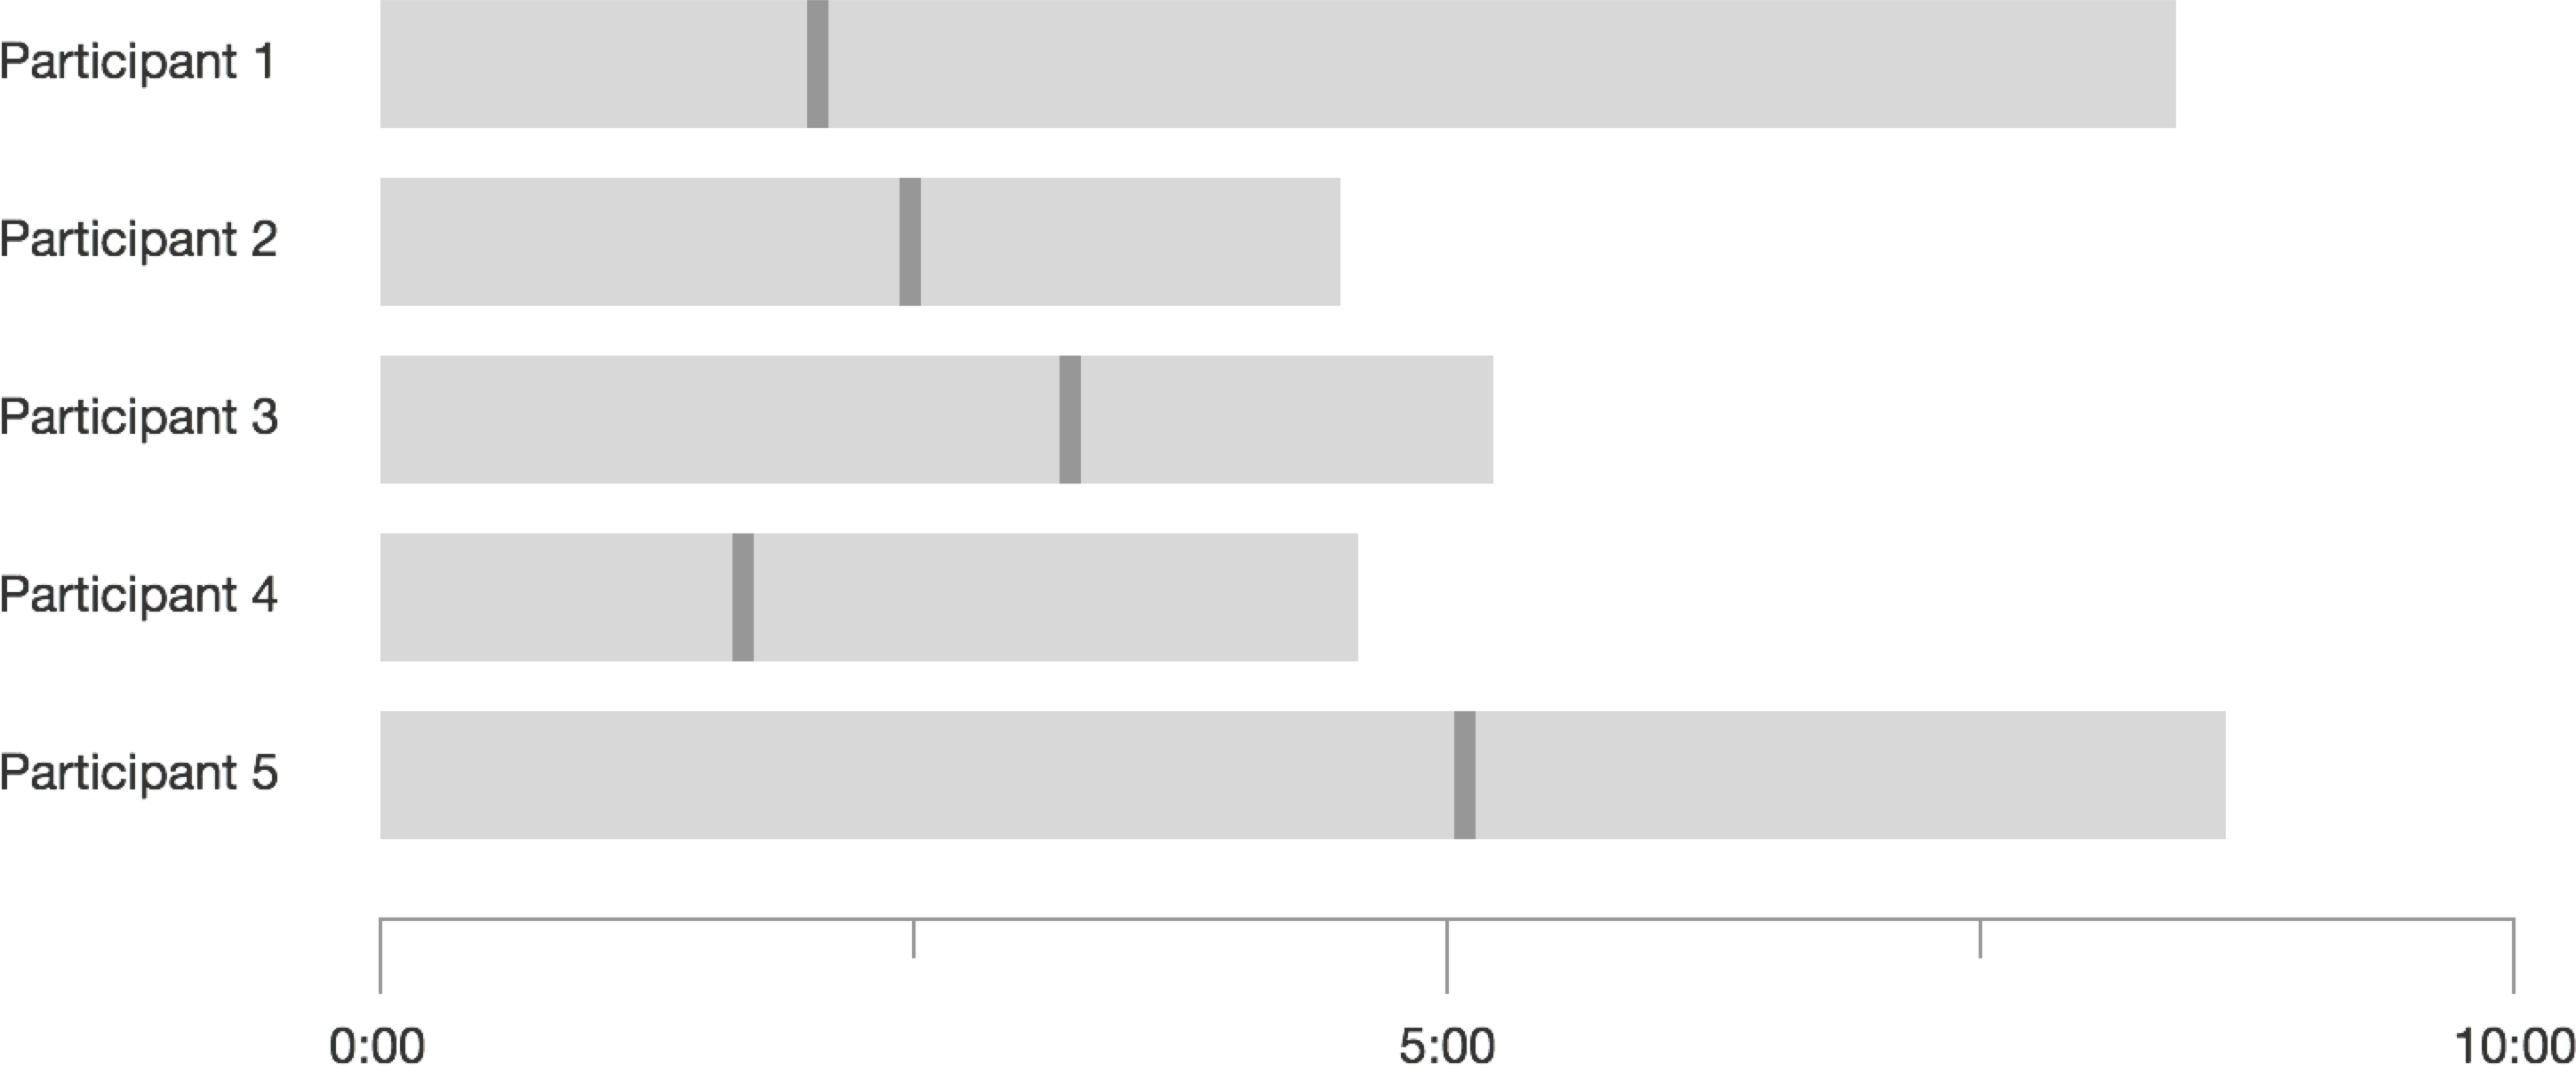
\includegraphics[width=\textwidth]{plot-time-till-branch-creation}
%  \caption{Total task completion time compared to discovery of branch creation button}
%  \label{fig:branch-creation-time}
% \end{figure}

% One factor that lead to this situation was that most users did not fully read the warning message, which told them they could not edit the main branch, but instead had to create a new one. The second factor, it seemed, was the missing label for the button that allowed the creation of a new branch. The button only consisted of a simple plus sign and a tooltip would explain more if the user hovered the button (Figure \ref{fig:create-new-branch-btn}). Some users, after exhausting all other options, turned to the last available option. Others accidentally hovered the button and thus discovered the feature.

% \begin{figure}[h!]
%  \centering
%  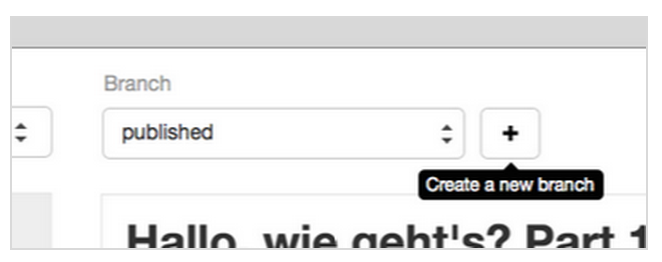
\includegraphics[width=6cm]{create-new-branch}
%  \caption{The branch selection next to the create-new-branch button}
%  \label{fig:create-new-branch-btn}
% \end{figure}

% Another problem was that some participants could not figure out how they could allow a colleague to review their edits. This is also reflected in the task completion percentage shown in Table \ref{table:task-completion-rate}. This issue seemed to be connected to bad naming (some users misinterpreted the \textit{back to editor button}) and an overlooked input field (\textit{reviewer} on pull request view). Furthermore, one user had a wrong mental model of the system in that she assumed the colleague who sent her the link would be informed about changes automatically.

% \subsubsection{Scenario 2}
% This scenario presented almost no problems to the participants. This is reflected by the low error rate, the short time needed for performing the tasks and the 100\% completion rate (Table \ref{table:task-completion-rate}). The three users who made zero errors while performing the tasks were drawn to the pull request view by the number indicator next to the button (Figure \ref{fig:number-indicator-pr}). The other two users struggled, because the concept of a pull request was meaningless to them, even though one of them had created one during the previous scenario. Both started by selecting folders in the main navigation and then went on to discover the right functionality through trial and error (“I have no idea, I’m just clicking through”). Once these users discovered the pull request view they were able to finish the task without major problems like the other participants.

% \begin{figure}[h!]
%  \centering
%  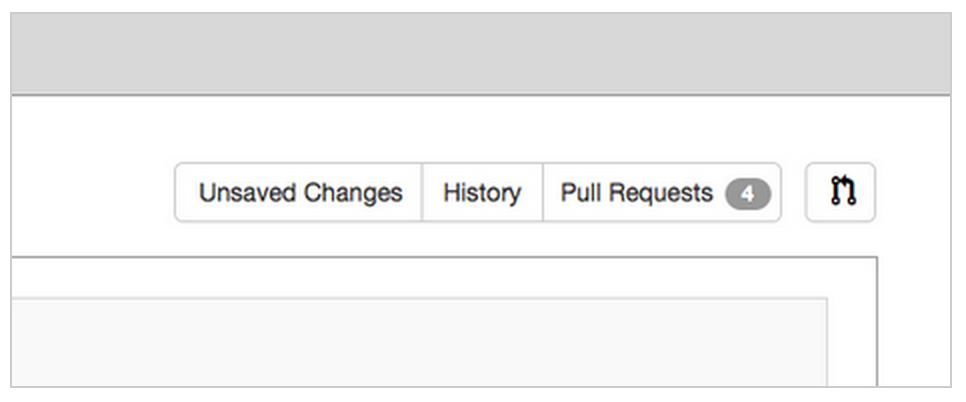
\includegraphics[width=9cm]{number-indicator-pr}
%  \caption{Number indicator next to the pull request button}
%  \label{fig:number-indicator-pr}
% \end{figure}

% \subsubsection{Scenario 3}
% This scenario, out of all scenarios, challenged participants the most. This can be seen in the high error rates (4.2 on average) and the time needed for completing the scenario, which was the highest of all scenarios. The first obstacle users encountered was that the changes could not be found in the list of pull requests as in the previous scenario, but instead in the history. During the post-session interviews some users stated, that the difference between the two was not clear. This could be due to the similarity of the two concepts. The history is a list of saved changes whereas a pull request is a request to integrate a set of changes into a different branch. But both are lists of changes, which could explain the confusion.

% The second major problem, which was even more severe, was that most users struggled to find the missing translation. This was partly due to confusion that was caused by the difference view (Figure \ref{fig:difference-view}). Users mistook the left column, which represents the old state of the data, for the missing translations. The other contributing factor was that users had to make an abstraction from the difference view to the list of items that were presented to them inside the editing view (Figure \ref{fig:missing-translation}). Those users that solved the task realized that a missing translation would not show up in the list of changes and thus they had to use the editing view to navigate to the respective item. User who did not complete the task (2 of 5) failed to make this connection.

% \begin{figure}[h!]
%  \centering
%  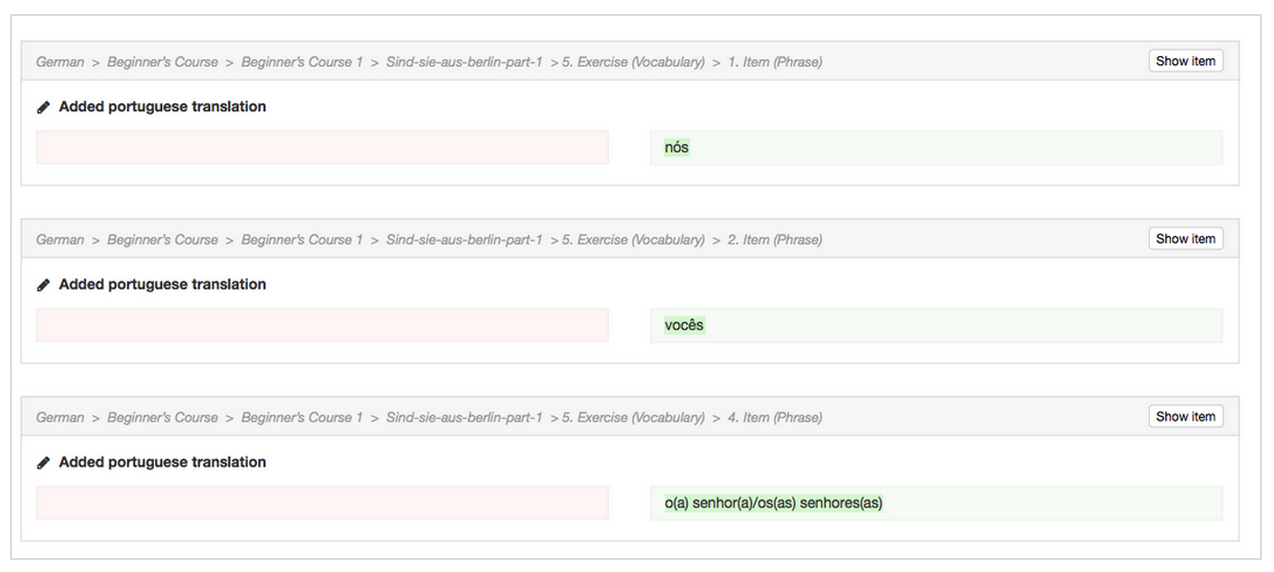
\includegraphics[width=\textwidth]{difference-view}
%  \caption{Difference view as presented to the user when inspecting changes}
%  \label{fig:difference-view}
% \end{figure}

% \begin{figure}[h!]
%  \centering
%  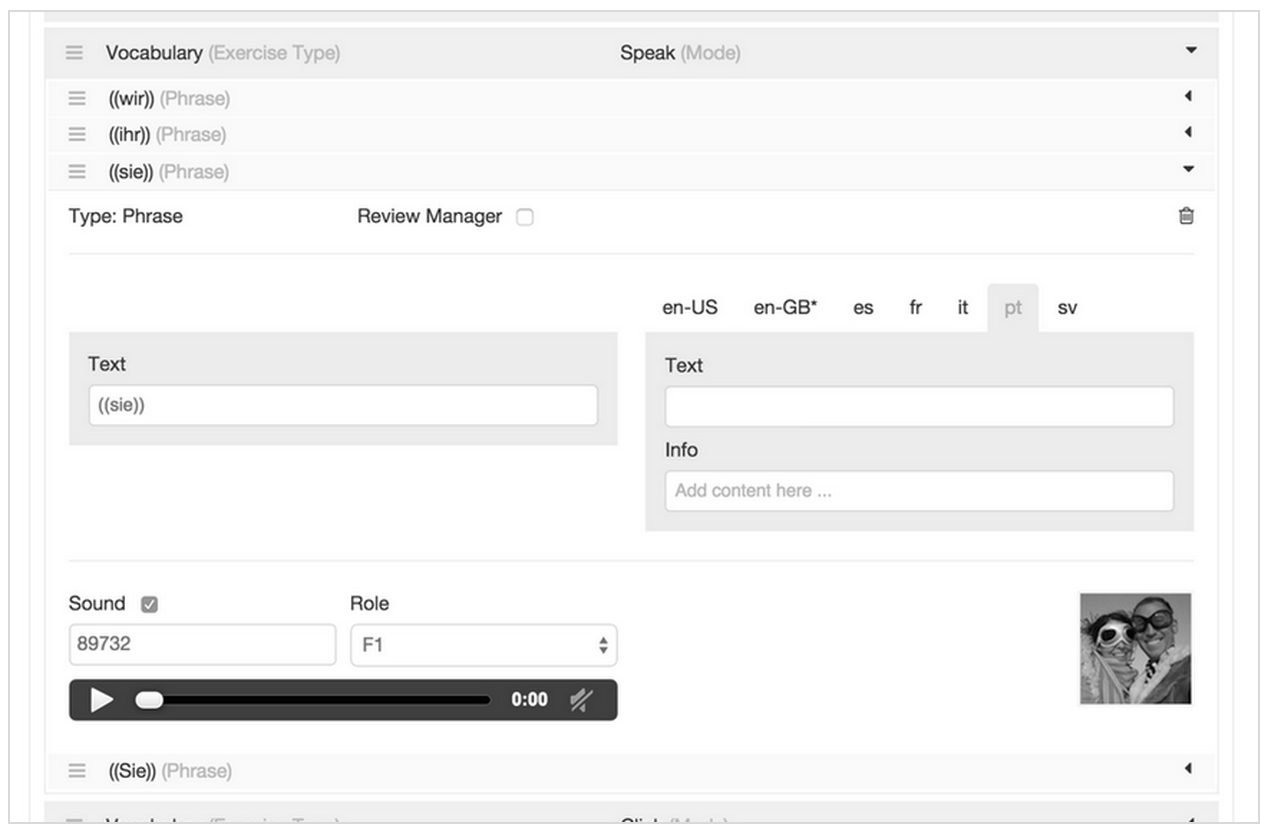
\includegraphics[width=\textwidth]{missing-translation}
%  \caption{Expanded item with missing translation}
%  \label{fig:missing-translation}
% \end{figure}

% I left out the recommendations/possible solutions -> maybe they could become part of each scenario?

\subsection{Conclusion} \label{sec:summary-usability-problems}
Concluding one could say that a long list of diverse usability issues has been identified. A number of severe issues prevented users from finishing their tasks, especially in Scenarios 1 and 3. This is also reflected in the somewhat low task completion rates for these scenarios.
Furthermore, using central features, such as branching and saving posed some serious problems, which reflected on the entire system. Last but not least, the use of technical terminology (e.g. branch or pull request) prevented some users from forming an accurate mental model of the system. But, despite these flaws, a majority of users still succeeded in reaching their goals, which is more important than having an accurate understanding of the underlying concepts, which will probably improve over time.

Nevertheless, there are many things that need to be improved for the next iteration of the interface. The following chapter looks at one aspect of that: the terminology used within the interface. After that, Chapter \ref{chapter:design-second-iteration} presents how the discovered issues were resolved and translated into a new interface design.


%During Scenario 1, especially the first part, creating a new branch, was a difficult hurdle for almost all users. This might be due to the fact that this approach was completely new to all participants, since none of them had used version control before. This problem was further intensified by the fact that users did not fully read the warning popup.

%Solutions for this problem, as described in the section above, are rephrasing the warning or offering a direct link to the branch creation view.

%Another issue, that most users had, is the separation of editing and saving. Even though some users stated that it is advantageous to get an overview of changes before saving, all of them were looking for a save button at the bottom of the editing view. It took them a while to locate the “unsaved changes” button at the top. The decoupling of saving and editing is an important feature that allows bundling changes into a coherent edit (which makes the history more valuable). Therefore, in order to keep this feature, a compromise needs to be found between offering users a familiar save and edit workflow while at the same time providing them the enhanced VCS capabilities.

%A big question mark is still how users can be introduced to the more complex version control features. During the post-session interviews it became clear that most participants had no real understanding of branches or pull requests. Furthermore, the difference between history and pull requests was not really clear.


%Nevertheless, a better understanding could probably be achieved through an improved naming instead of just using the existing Git terminology.

% \subsection{Recommendations}
% Based on the results of this user study a few recommendations were drafted. These acted as broad guidelines for the design of the next prototype.

% \begin{itemize}
%   \item Offer a short interactive tutorial that introduces new users to the most important version control concepts
%   \item There should be a direct path from the master branch warning to the branch creation view (or at least a better description: “create a new branch first” could be the headline for example)
%   \item Button order should reflect temporal sequence in which functions are used: branch creation/selection - saving changes - getting an overview of changes (history) - merging branches
%   \item Offer a save button at the bottom of the editing view which either leads to the unsaved changes view or lets users save without reviewing the changes again (lesson based)
%   \item Names for the most important features could be reconsidered (Focus Group)
%   \item Item list should be numbered
%   \item Evaluate whether providing more context within change overview is feasible (images, speaker role)
%   \item Highlight which item actually is selected, what changed (after coming from the change overview)
% \end{itemize}



